\documentclass[12pt]{article}
\usepackage[a4paper]{geometry}
\usepackage[myheadings]{fullpage}
\usepackage{fancyhdr}
\usepackage{lastpage}
\usepackage{graphicx, wrapfig, subcaption, setspace, booktabs}
\usepackage[T1]{fontenc}
\usepackage[font=small, labelfont=bf]{caption}
\usepackage{fourier}
\usepackage[protrusion=true, expansion=true]{microtype}
\usepackage[spanish]{babel}
\usepackage{sectsty}
\usepackage{url, lipsum}
\usepackage{hyperref}
\usepackage{fancyhdr,lipsum}


\hypersetup{
    colorlinks=true, %set true if you want colored links
    linktoc=all,     %set to all if you want both sections and subsections linked
    linkcolor=blue,  %choose some color if you want links to stand out
}
\urlstyle{same}


\newcommand{\HRule}[1]{\rule{\linewidth}{#1}}
\onehalfspacing

\setcounter{secnumdepth}{2}
\setcounter{tocdepth}{5}

%-------------------------------------------------------------------------------
% HEADER & FOOTER
%-------------------------------------------------------------------------------
\pagestyle{fancy}
\fancyhf{}
\setlength\headheight{15pt}
\fancyhead[L]{SSII}
\fancyhead[R]{\uppercase{Instalación de Sistemas Operativos}}
\fancyfoot[R]{Page \thepage\ of \pageref{LastPage}}

%-------------------------------------------------------------------------------
% TITLE PAGE
%-------------------------------------------------------------------------------

\begin{document}

\title{ \normalsize \textsc{SISTEMAS INFORMÁTICOS\\
I.E.S FRANCISCO DE LOS RÍOS}
		\\ [2.0cm]
		\HRule{0.5pt} \\
		\LARGE \textbf{\uppercase{Instalación de Sistemas Operativos}}
    \HRule{0.5pt} \\
    \HRule{2pt} \\ [0.5cm]
    %\normalsize  \vspace*{10\baselineskip}
    \LARGE \textbf{\uppercase{WINDOWS 10}}
    \HRule{2pt} \\ [0.5cm]
    \normalsize  \vspace*{2\baselineskip}
    }

\author{
        Trabajo realizado por: \\
		Antonio Muñoz Cubero
	    \normalsize  \vspace*{4\baselineskip}
		}
\date{\textbf{01 de Febrero de 2021}}
\newpage
\maketitle
\newpage

%-------------------------------------------------------------------------------
% Table of Content
\tableofcontents
\newpage
%-------------------------------------------------------------------------------

%-------------------------------------------------------------------------------
% Section title formatting
\sectionfont{\scshape}
%-------------------------------------------------------------------------------






%-------------------------------------------------------------------------------
% BODY
%-------------------------------------------------------------------------------


    \section*{Introducción}
      En el transcurso de esta práctica seguiremos los pasos adecuados para que la Instalación del sistema 
      operativo, en este caso \textbf{Windows 10} se realice de manera satisfactoria. También hemos de cumplir 
      una serie de criterios para la correcta realización de la misma, que son los siguientes.
      \begin{itemize}
        \item Se realizará la configuración del hardware virtual según los requisitos del sistema invitado 
        (memoria RAM y tamaño de disco) para ello se buscará información en la página Web de Microsoft 
        para consultar cuáles son dichos recursos mínimos.
        \item  El nombre del sistema o del usuario en su defecto (durante la instalación) será igual al nombre 
        de usuario del alumno/a en moodle. (Captura de pantalla).
        \item Omitir la creación de cuenta en Microsoft mediante correo electrónico (Captura de pantalla).
        \item La conexión de red será de tipo NAT o Red NAT con configuración IP automática.
        \item Una vez instalado comprobar que el sistema está actualizado, pero no instalar las actualizaciones. 
        (Captura de pantalla).
      \end{itemize}
      También he de destacar que la imagen que usaré para la instalación del sistema operativo fue proporcionada por el 
      profesor.

    \newpage
    
    \section{Creacion de la máquina virtual}
      El primer paso de esta práctica es la creación y configuración de una máquina virtual adecuada para la instalación 
      del sistema operativo que vayamos a utilizar, en nuestro caso usaremos \textbf{Windows 10}. Para ello, abrimos 
      nuestro programa de virtualización y le damos a añadir una nueva máquina virtual y nos desplegará el siguiente menú
      en el caso que usemos \textit{virtual box}
      \begin{figure}[h]
        \centering
        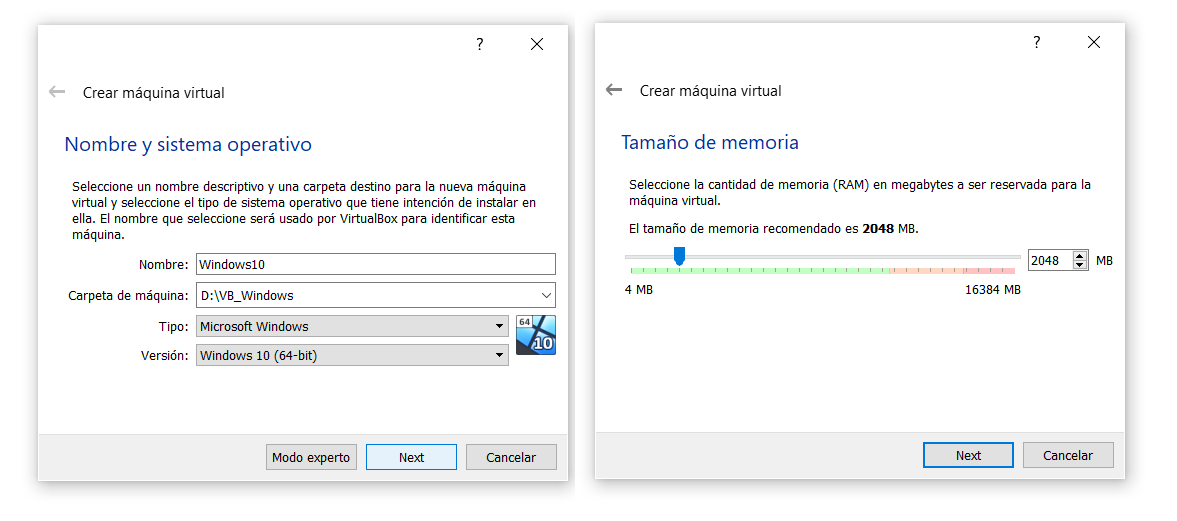
\includegraphics[scale = 0.5]{img/windows_install_1.png}
        \caption{Creacion de la máquina virtual.}
        \label{Windows1}
      \end{figure}

      La configuración de la máquina virtual está hecha acorde a los requisitos mínimos del sistema, que previamente hemos 
      buscado. Tras esto, solo hemos de confirar la máquina virtual siguiendo dichos requisitos.

      \begin{figure}[h]
        \centering
        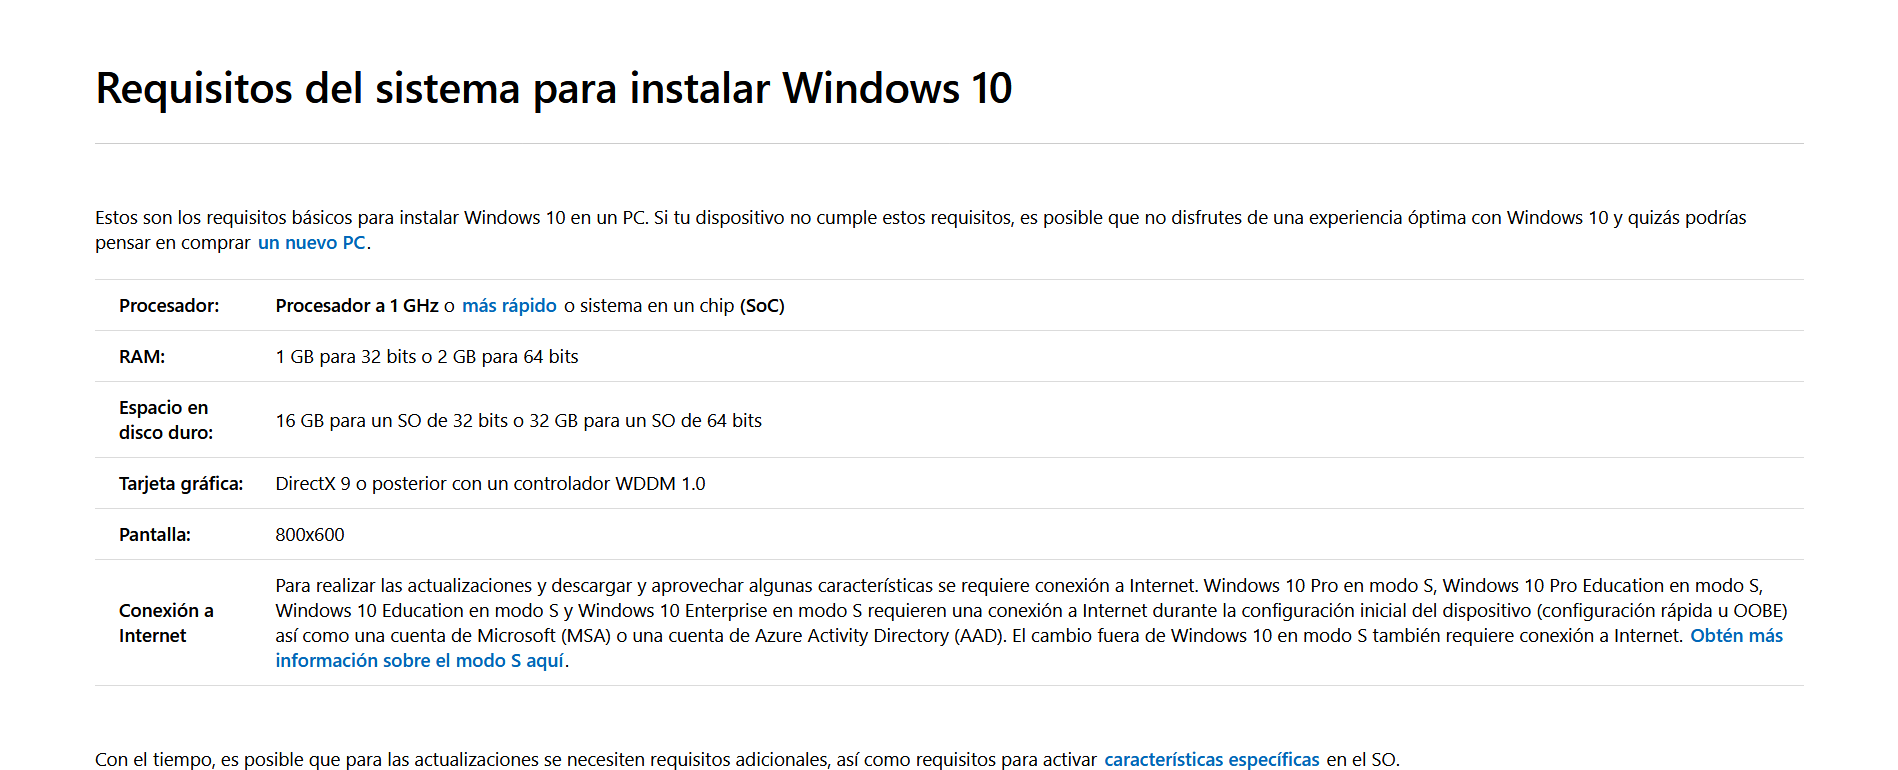
\includegraphics[scale = 0.4]{img/requisitos_w10.png}
        \caption{Requisitos mínimos Windows 10.}
        \label{requisitos}
      \end{figure}

      \newpage

      Ahora simplemente, rellenamos los campos que nos piden con los parámetros adecuados para el correcto 
      funcionamiento del sistema.

      \begin{figure}[h]
        \centering
        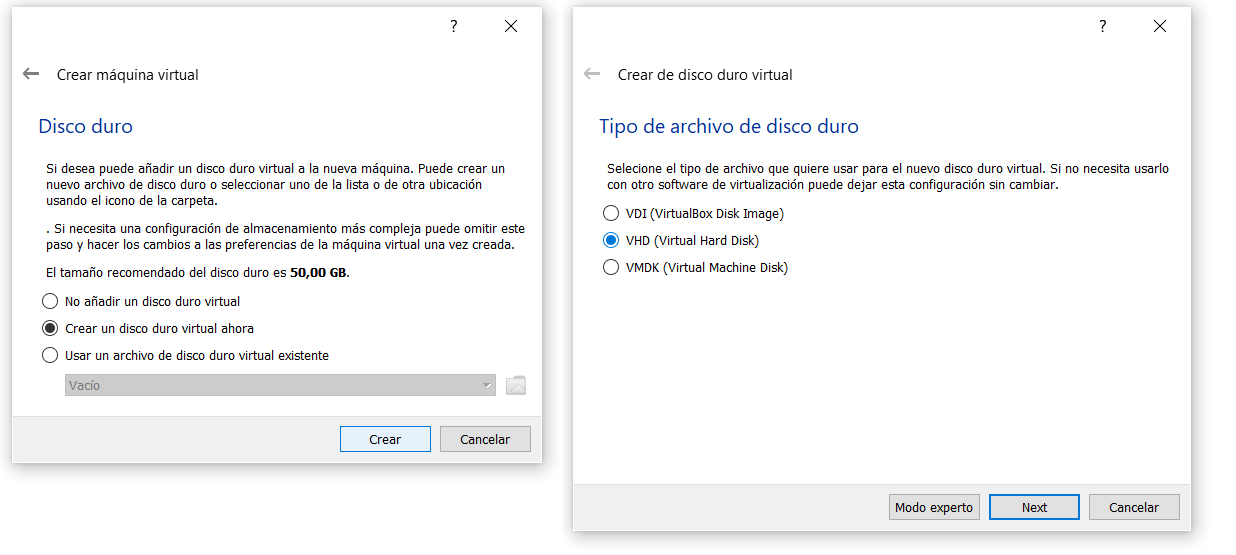
\includegraphics[scale = 0.5]{img/windows_install_3.png}
        \caption{Creacion de la máquina virtual.}
        \label{Windows2}
      \end{figure}

      \begin{figure}[h]
        \centering
        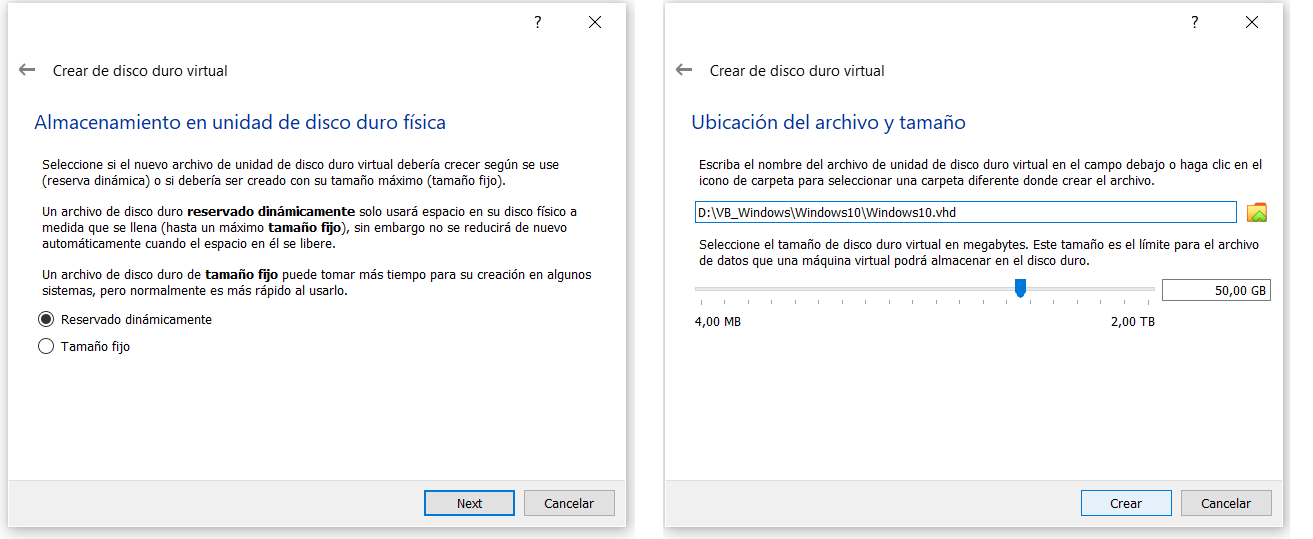
\includegraphics[scale = 0.5]{img/windows_install_5.png}
        \caption{Creacion de la máquina virtual.}
        \label{Windows3}
      \end{figure}
    
      Una vez seguidos estos pasos, nuestra máquina virtual estará creada y lista para su funcionamiento. Ahora 
      nos queda montar la imagen y proceder a la instalación.
    
    
    
    
    
    
    
    
    
    
    \newpage

    \section{IMÁGENES}
    \listoffigures
      
\end{document}